%!TEX root = ../thesis.tex
%*******************************************************************************
%****************************** Third Chapter **********************************
%*******************************************************************************
\chapter{An analysis of the seasonal cycle of aerosol radiative forcing in UKESM1}

% **************************** Define Graphics Path **************************
\ifpdf
    \graphicspath{{Chapter4/Figs/Raster/}{Chapter4/Figs/PDF/}{Chapter4/Figs/}}
\else
    \graphicspath{{Chapter4/Figs/Vector/}{Chapter4/Figs/}}
\fi


\section*{Abstract}

- despite extensive measurement campaigns in the 1990s to quantify the changes in SO2 and its oxidation and recent development on the radiative effects of aerosols, there has been no studies that link the seasonality of oxidation to radiative effects.
- This chapter addresses the seasonality of said so2 oxidation and its effects on radiative effects.
- changes in the pathway of oxidation change the aerosol size distribution over the year, which impacts its lifetime in the atmosphere as well as its interaction with clouds.
- The UKESM 1 simulates aerosol number and mass independently, thus is capable of simulating the seasonal variation of aerosol properties required.

\section{Introduction}

From the previous chapter, I concluded that \ce{O3} and \ce{CH4} slightly modify \ce{SO2} oxidation by changing the available oxidant. In addition to the SLCFs, oxidants also show seasonal and diurnal cycles. Multiple field experiments show that \ce{SO2} conversion rate to sulfate by \ce{SO2 + OH} increases by a factor of 1 between summer and winter \cite{meagherSeasonalVariationAtmospheric1983}. A model study also indicates that the oxidant levels and respective oxidation exhibit a seasonal cycle \cite{feichterSimulationTroposphericSulfur1996}. This poses the question of whether the change in the oxidation pattern due to seasonality affects aerosol radiative effects.


According to field studies using instrumented aircraft sampling down-wind air from coal-fired power plants between 1975-1978, the gas-phase \ce{SO2} oxidation has a strong seasonal cycle \cite{meagherSeasonalVariationAtmospheric1983}. The oxidation rate varies from a winter low of \num{1.5E-3} \unit{\per\hour} to a summer high of \num{1.3E-2} \unit{\per\hour}. 

conversion rate, $k(SO_4^{2-})$, is calculated from
\begin{equation}
k(SO_4^{2-}) = \frac{[SO_4^{2-}]}{([SO_2]+[SO_4^{2-}])t}
\end{equation}
where t is the plume travel time. The plume was sampled at several downwind distances.

In the same study, correlation analysis was also performed between conversion rate and other parameters, including type of power plant and location, time of day, solar intensity, temperature, background O3 concentration, relative humidity, and specific humidity. Only specific humidity and temperature correlate significantly with the conversion rate. This work suggested that the correlation is due to the seasonal trend rather than a direct relationship of the variable. \ce{SO2} conversion rate at noon at 35 degrees N from a model study also suggests that there is a 4-fold increase in \ce{SO2 + OH} oxidation between summer and winter which agrees with the observation as shown in Fig. \ref{fig:ch4:meagher1983}.

\begin{figure}
    \centering
    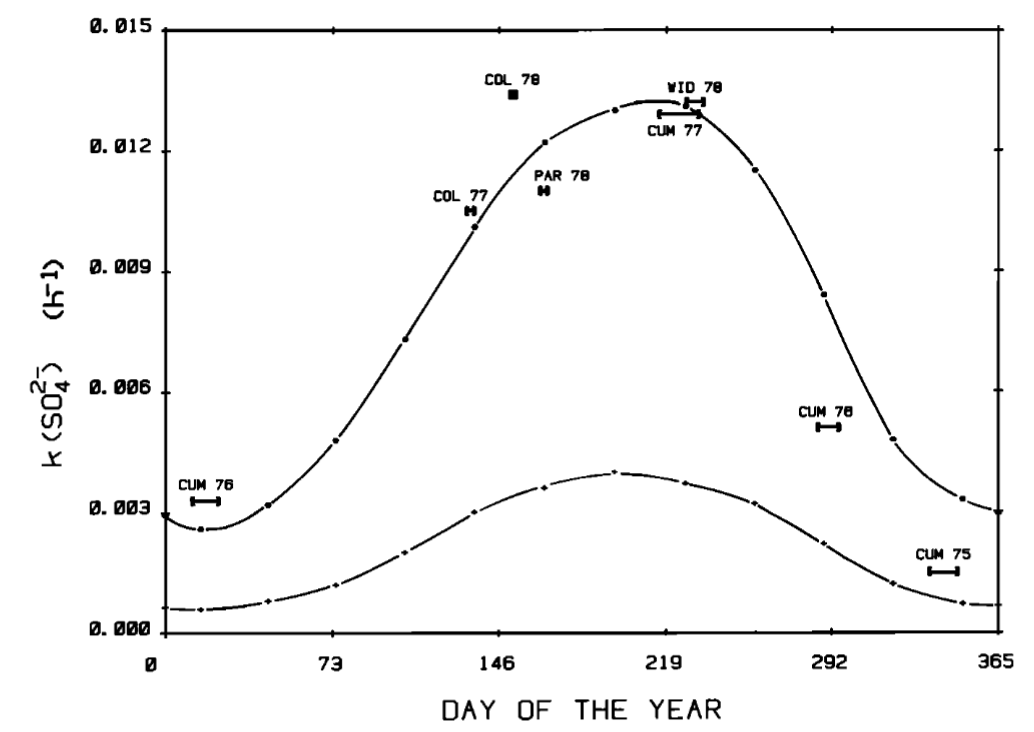
\includegraphics[width=0.7\linewidth]{Chapter4/Figs/meagher1983.png}
    \caption{Average rate of \ce{SO2} conversion to \ce{SO_4^{2-}} measured at different power station plumes. Also shown in this figure are the noontime (top curve) and diurnal average (bottom curve) \cite{meagherSeasonalVariationAtmospheric1983}}
    \label{fig:ch4:meagher1983}
\end{figure}

\citet{eatoughConversionSO2Sulfate1994} noted that \ce{SO2 + OH} is the most important and most rapid during daytime and in summer due to more OH concentration from photochemical reactions. However, \ce{H2O2} oxidation becomes more important during nighttime or when atmospheric water droplets are present such as in clouds and fog \cite{eatoughConversionSO2Sulfate1994}. 

Field studies suggest that the aqueous-phase concentration of the oxidant and the reaction kinetics factors, including cloud droplet pH and temperature, are the two important factors influencing the oxidation process \cite{eatoughConversionSO2Sulfate1994}. \ce{SO2} in the gas phase gets dissolved into water droplets along with its important oxidants including O3 and H2O2. Both \ce{O3} and \ce{SO2} are moderately soluble in the pH range 3-6, which is the typical atmospheric acidity. Most of the dissolved SO2 will be present as \ce{HSO_3^-} with the concentration of \num{e-4} M. Atmospheric mixing ratio of tropospheric \ce{O3} generally falls in the range between 50-100 ppb, resulting in approximately \num[]{e-9} M. \ce{H2O2} is very soluble, with the atmospheric mixing ratio between 0.1-5 ppb, aqueous concentration is expected at about \num[]{e-4} M \cite{eatoughConversionSO2Sulfate1994}.


Another model study shows a global SO2 oxidation trend for gas- and aqueous-phase oxidation \cite{feichterSimulationTroposphericSulfur1996}.

\begin{figure}
    \centering
    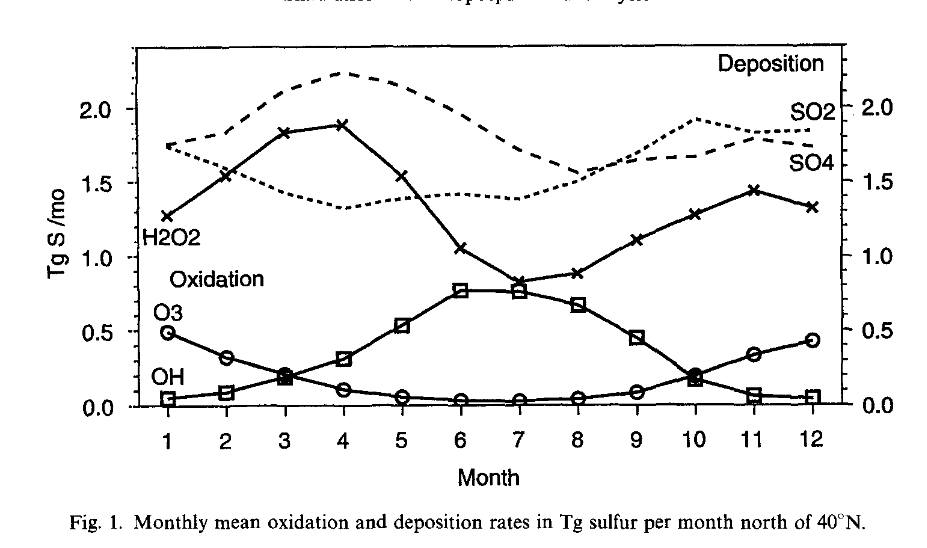
\includegraphics[width=0.7\linewidth]{Chapter4/Figs/feitcher1996.png}
    \caption{Monthly mean \ce{SO2} oxidation and deposition from a modelling study. \cite{feichterSimulationTroposphericSulfur1996}}
    \label{fig:feichter1996}
\end{figure}


Most studies in the literature focus on the effects of SO2 oxidation on air pollution especially on particulate matter concentration and acid rain \cite[e.g.][]{eatoughConversionSO2Sulfate1994}. 

- despite extensive measurement campaigns in the 1990s to quantify the changes in SO2 and its oxidation and recent development on the radiative effects of aerosols, there has been no studies that link the seasonality of oxidation to radiative effects.

- \citet{brodowskyAnalysisGlobalAtmospheric2024} also compared the sulfur budget across many ESMs but the focus was on stratospheric sulfate aerosols and there is no discussions on tropospheric sulfate aerosol seasonal trends nor radiative effects.

This means SO2 emission in summer could lead to more aerosol number production compared to winter. As aerosol-cloud interaction depends more strongly on the change in aerosol number, one could also hypothesise that the aerosol-cloud interaction would be stronger during summer due to more aerosol numbers. While both measurement and modelling studies have confirmed the seasonal cycle of SO2 oxidation, there has not been a detailed study of how this change in aerosol formation would affect cloud formation in the historical period. 

The UKESM1 can simulate both aerosol mass and number independently, making it one of the most robust climate models regarding aerosol simulation. GLOMAP-mode which is the aerosol module used in UKESM1 simulates both soluble and insoluble aerosols in four modes: nucleation, Aitken, accumulation and coarse and different aerosol types: sulfate, sea salt, organic, dust and black carbon. It also simulates interaction between modes such as coagulation and condensation as well as wet and dry deposition. This makes the UKESM1 a useful tool for studying the aerosol properties in different seasons.

Changes in aerosol formation in different seasons may lead to changes in aerosol-cloud radiative effects. This chapter asks how the seasonal oxidant changes affect aerosol formation and the climate system.



\section{Methods}

\subsection{Sulfate production rates in the UKESM1}
\label{ch4:sec:so4-prod-rate}
The termolecular rate constant of \ce{SO2 + OH}, reaction \ref{ch1:eq:so2-oh}, depends on the concentration of air and temperature via the following relationship. The constants are given in Table \ref{ch4:tab:so2-oh-reaction-consts}.
\begin{align}
    k_0 &= k_1 \left(\frac{T}{300}\right)^{\alpha_1} \exp{(-\beta_1/T)} \\
    k_\infty &= k_2 \left(\frac{T}{300}\right)^{\alpha_2} \exp{(-\beta_2/T)}\\
    k_{([M],T)} &= \left( \frac{k_0[M]}{1+\frac{k_0[M]}{k_\infty}}\right) F_c^{\left\{ 1+\left[ \log_{10} \left( \frac{k_0[M]}{k_\infty}\right) \right]^2 \right\}^{-1}} 
\end{align}


\begin{table}[]
\centering
    \begin{tabular}{ccccccccc}
    \hline
    Reactants & Products & $F_c$ & $k_1$ & $\alpha_1$ & $\beta_1$ & $k_2$ & $\alpha_2$ & $\beta_2$ \\ \hline
    \ce{SO2 + OH} & \ce{SO3 + HO2} & 0.60 & 3$\times 10^{-31}$ & -3.3 & 0 & 1.5$\times 10^{-12}$ & 0 & 0 \\ \hline
    \end{tabular}
\caption{constants for \ce{SO2 + OH} reaction}
\label{ch4:tab:so2-oh-reaction-consts}
\end{table}

The aqueous-phase reactions in the UKESM1 require more information about cloud droplets and cloud droplet acidity as acidity determines the reaction rate of \ce{SO2 + O3} and \ce{SO2 + H2O2} \citep{seinfeldAtmosphericChemistryPhysics2016}. Once the reaction rates are determined from Equations \ref{ch1:eq:so2-o3}--\ref{ch1:eq:so2-h2o2}, the in-cloud sulfate aerosol production is obtained from
\begin{align}
    \Delta S_{\mathrm{cloud}} = F \cdot \left( \dfrac{d[S(IV)]}{dt}\right) \cdot L \cdot N_a \cdot \frac{1}{\rho_w} \label{ch4:eq:in-cloud-sulfate-prod}
\end{align}
where $F$ is the cloud fraction, $ \dfrac{d[S(IV)]}{dt}$ is the aqueous-phase reaction rate, $L$ is the cloud liquid water content, $N_a$ is the Avogadro's constant, and $\rho_w$ is the density of water.

\section{Results and discussions}

This section shows, firstly, the seasonal cycle of aerosol effective radiative forcing. Then, I attempt to explain this phenomenon by analysing the annual cycle of oxidant, sulfate oxidation tendency, aerosol and cloud properties. Two time periods were chosen: 1980-1989 and 2005-2014. 



\subsection{seasonal cycle of \ce{SO2} emission and oxidants}

\ce{SO2} is oxidised in the gas phase with \ce{OH} and the aqueous phase with \ce{O3} and \ce{H2O2}. First, we investigate the oxidants' concentration and then the oxidation tendency.

\begin{figure}
    \centering
    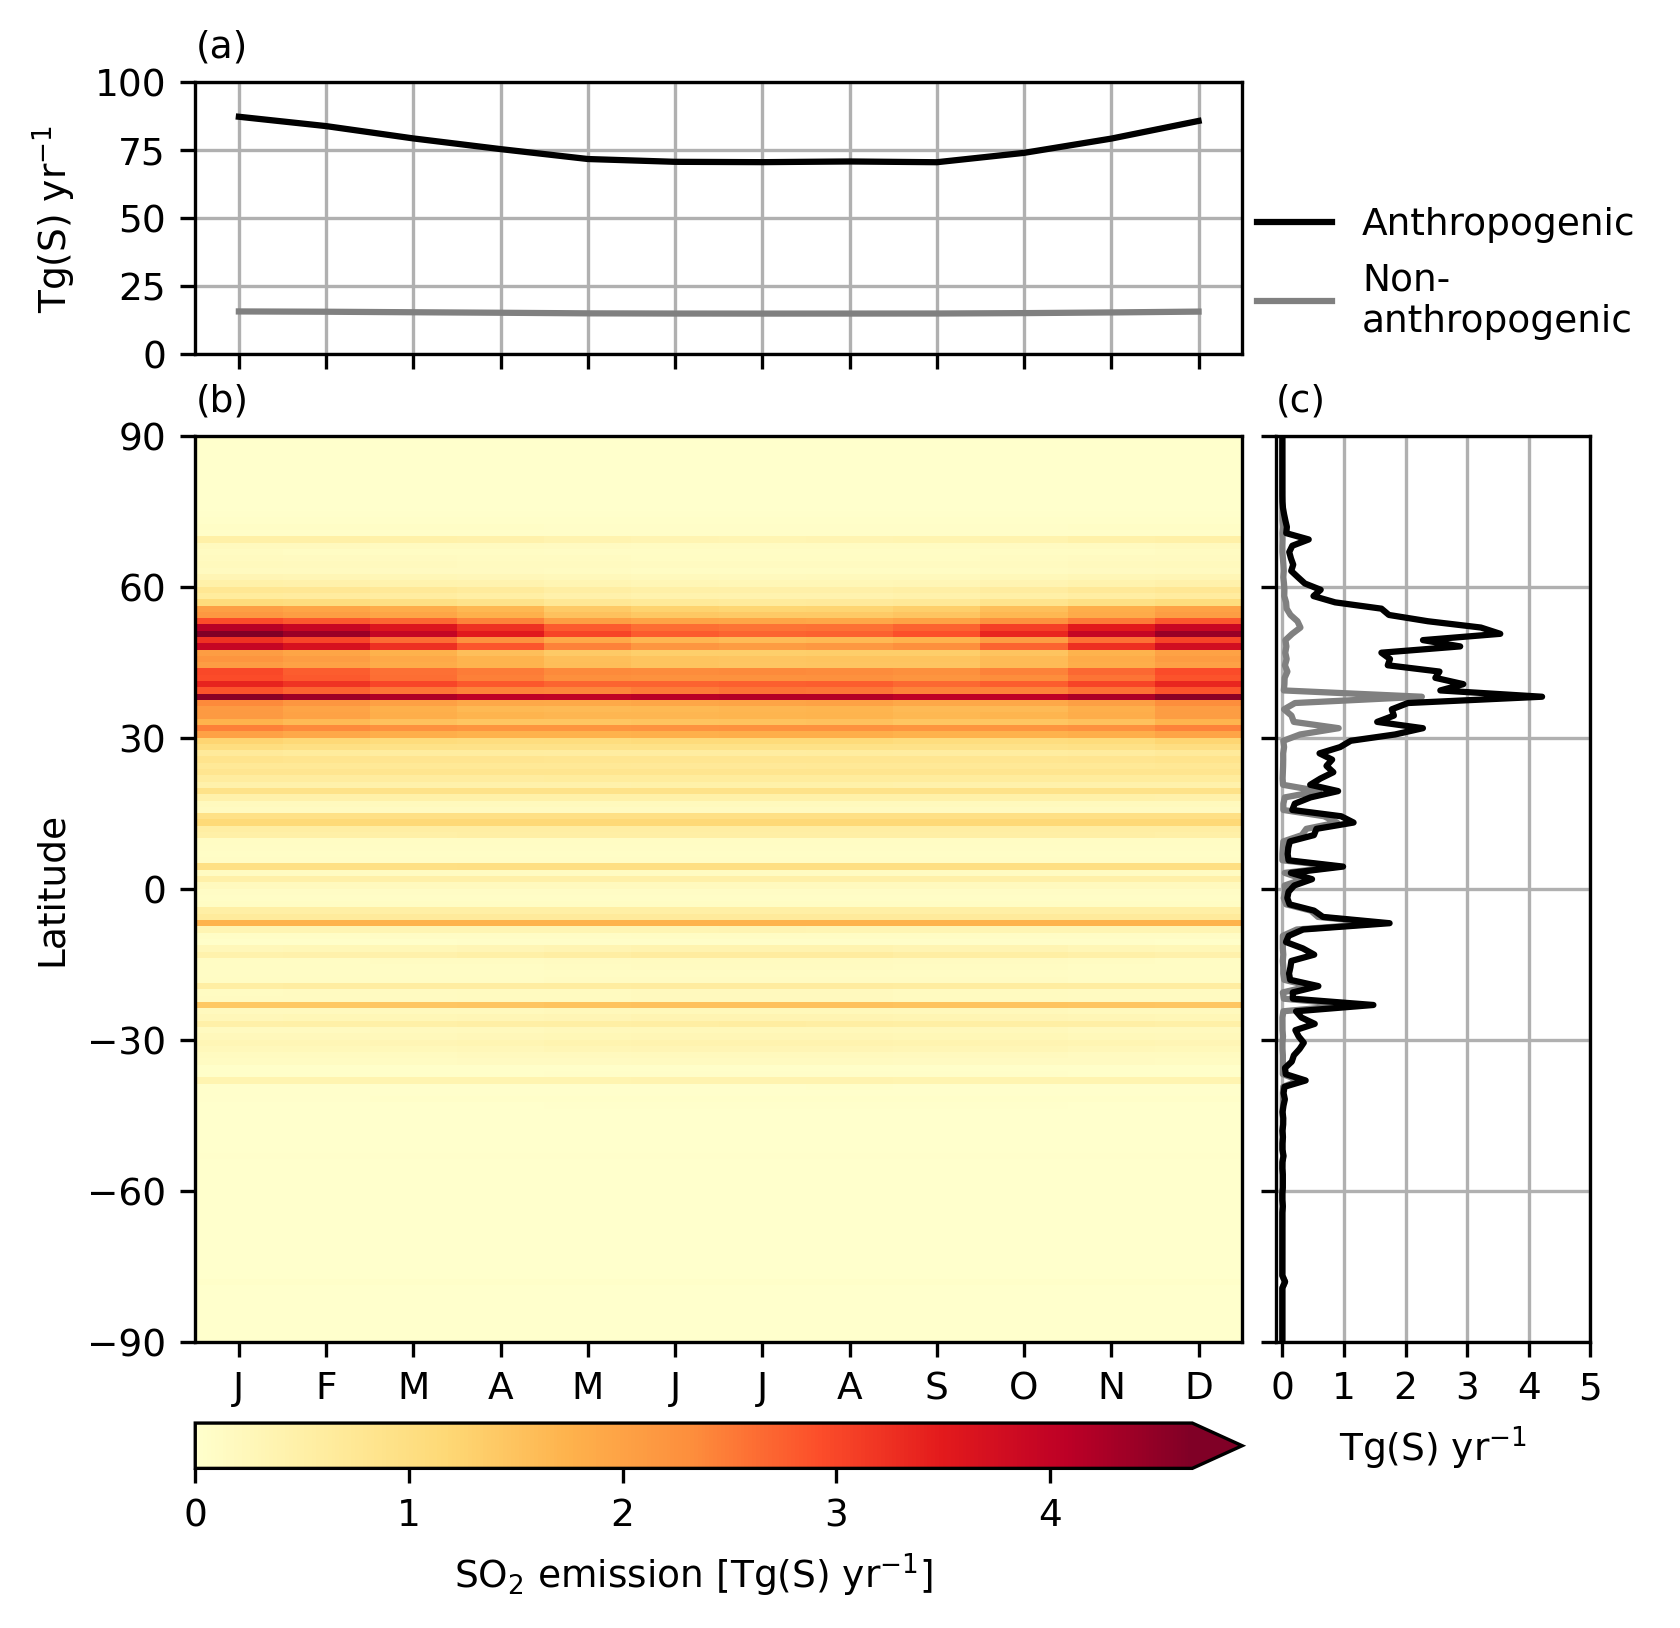
\includegraphics{Chapter4/Figs/emiso2_monthly_1980.png}
    \caption{\ce{SO2} emission between 1980 and 1989 as a function of month of year and latitude}
    \label{fig:ch4:seasonal-emission}
\end{figure}

Fig. \ref{fig:ch4:seasonal-emission} shows SO2 emissions between 1980 and 1989. SO2 emissions is higher in the boreal winter as more energy usage rises. The difference between summer and winter is approximately 12.5 Tg(S) yr$^{-1}$. Most emissions in this period come from fast-growing countries in the European regions and Northern America region, accounting for xx\% (Xx Tg(S) yr-1) of the annual mean of xx Tg yr-1. Also shown here is that only anthropogenic emissions exhibit a seasonal cycle.

OH, O3 and H2O2 are produced in the atmosphere with a strong correlation to the photolysis of O3 to form O1D. Concentrations reach maximum concentration during their respective hemispheric summer. SO2 concentration is localised near emission sources and peaks in winter where emission is higher as shown in Fig. \ref{fig:ch4:seasonal-emission}.

\begin{figure}
    \centering
    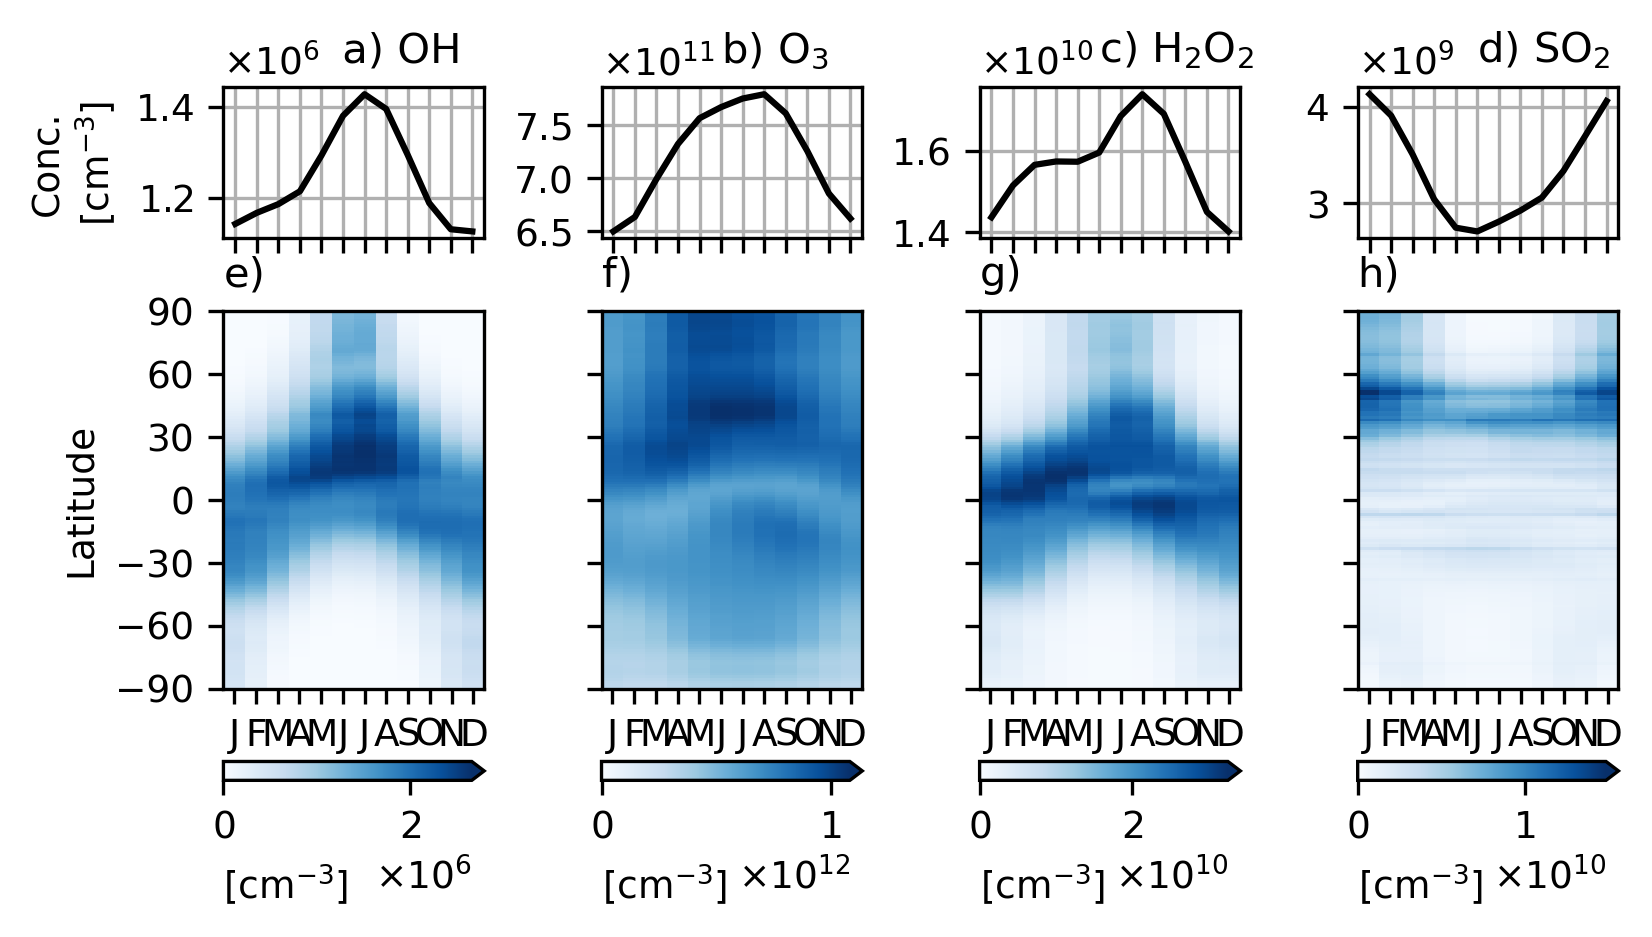
\includegraphics[width=\linewidth]{Chapter4/Figs/seasonal_oxidant_1980.png}
    \caption{Seasonal oxidant}
    \label{fig:ch4:seasonal-oxidants}
\end{figure}

% Discuss O3 production in the troposphere and its dependency on radiation
Discuss O3 production in the troposphere and its dependency on radiation

% Discuss the OH production via O1D+H2O
Discuss the OH production via O1D+H2O

% Discuss H2O2 production in the troposphere
Discuss H2O2 production in the troposphere

% Discuss SO2 loss via reaction with all the oxidants and also refer to emission seasonal cycle
Discuss SO2 loss via reaction with all the oxidants and also refer to the emission seasonal cycle

Thus, SO2 and its oxidants' concentration anticorrelate across time of year, with SO2 emission reaching maximum while its oxidants are minimised. With the knowledge of the behaviour of the oxidants in mind, we now explore the seasonal trends in oxidation.

\subsection{Seasonal cycle of oxidation}

Here we show the \ce{SO2} oxidation between 1980 and 1989 as a function of month of year and latitude.

\begin{figure}
    \centering
    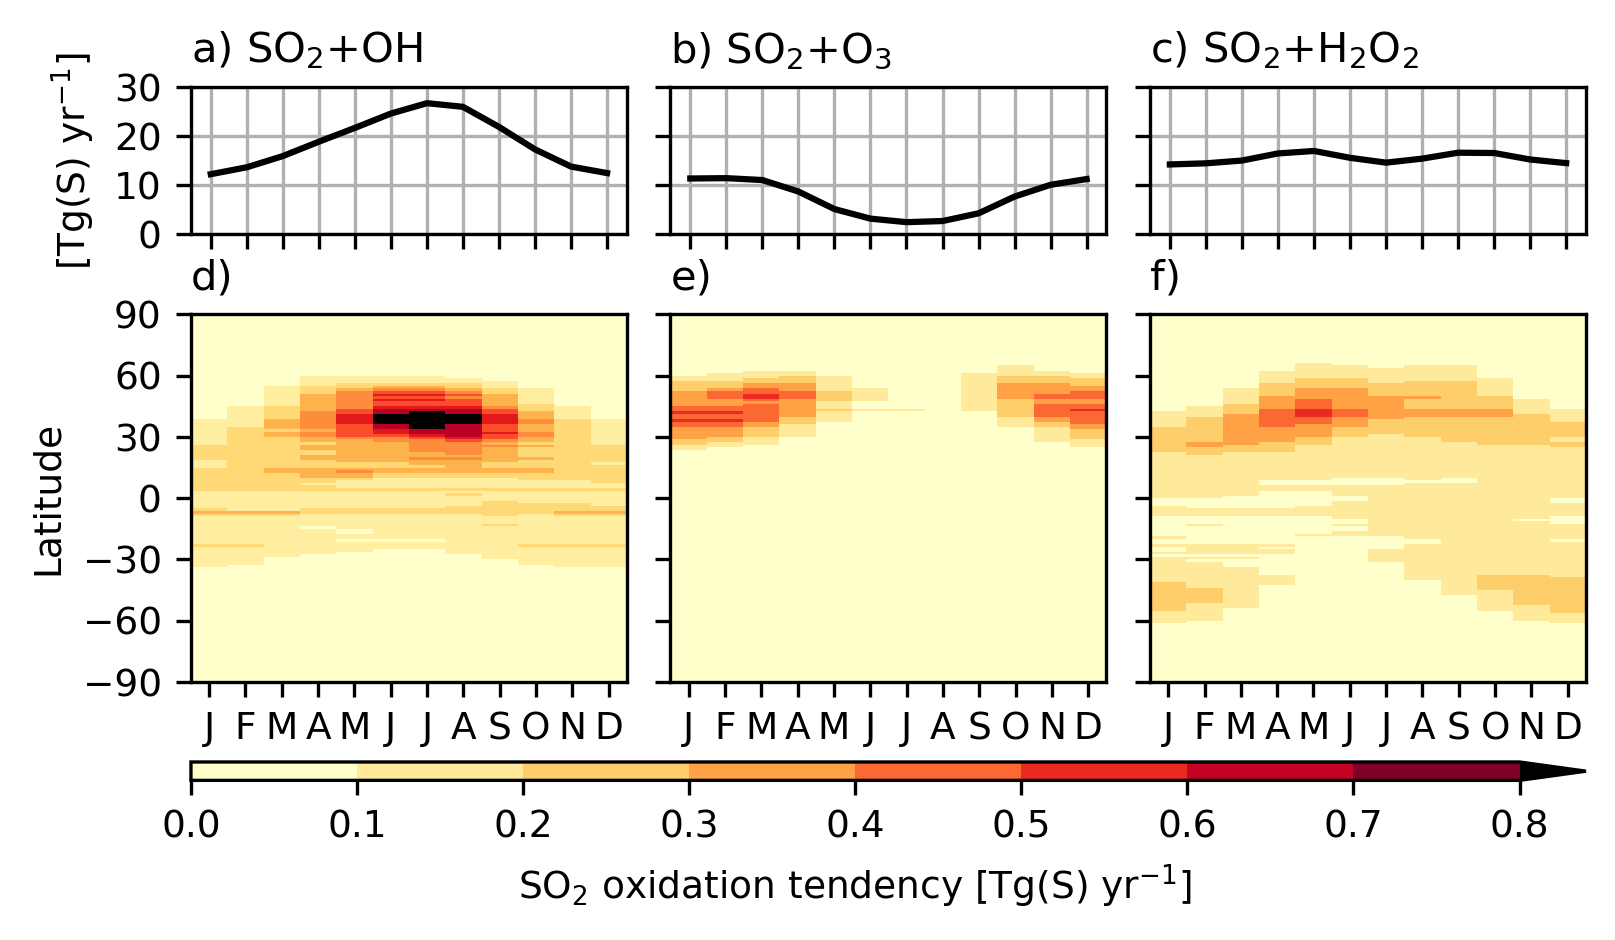
\includegraphics[width=\linewidth]{Chapter4/Figs/seasonal_oxidation_w_summary_histsst_1980.png}
    \caption[Seasonal cycle of oxidants]{Seasonal cycle of oxidants including a) OH, b) \ce{O3}, c) \ce{H2O2} and d) \ce{SO2}. e-g) shows the average oxidant concentration below 5 km between 1980 and 1989 }
    \label{fig:ch4:seasonal-oxidation}
\end{figure}

Fig.\ref{fig:ch4:seasonal-oxidation} show that \ce{SO2 + OH} peaks during boreal summer. This is expected as OH concentration is also high during the same period. However, for the aqueous-phase reactions, \ce{SO2 + O3} and \ce{SO2 + H2O2}, the oxidation tendencies do not follow the trends of their respective oxidants. This implies that the concentration levels of \ce{O3} and \ce{H2O2} are not the limiting factor for aqueous-phase oxidation. 



Unlike the gas-phase reactions, both \ce{SO2 + O3} and \ce{SO2 + H2O2} occur in water droplets. The reaction rate is thus controlled by the amount of water droplets present in the model as well as the solubility of the oxidant into the droplets, which is also controlled by temperature. The next section explores the sensitivity of all oxidation pathways to temperature, cloud droplet pH and also cloud fraction which determines the fraction of cloud in the model grid box.

% Insert cf x lwc here


\subsubsection{Sensitivity of \ce{SO2} oxidation}

In this section, we aim to quantify the sensitivity of oxidation to cloud fraction and oxidant levels from the theoretical point of view. A detailed description of sulfate chemistry is described in Section \ref{ch1:so2-oxidation}. 

% Describe gas-phase parameters
Describe gas-phase parameters: oxidants, T, P

% Describe aqueous-phase parameters
Describe aqueous-phase parameters: oxidants, T, P, pH, cf, lwc
The aqueous-phase reaction rate is determined from the amount of cloud water droplets as described in Section \ref{ch4:sec:so4-prod-rate}. 

% Describe the oxidant values from different measurement campaigns
Table \ref{ch4:tab:sensitivity-test} describes the oxidant values from different measurement campaigns. Describe the time dependence of oxidants including the diurnal cycle.

\begin{table}[]
\centering
\begin{tabular}{p{1.8cm} p{1cm} p{1.25cm} p{1cm} p{1cm} p{0.8cm} p{1cm} p{1cm} p{1cm} p{1cm}}
\toprule
 & \ce{SO2} [ppb] & OH conc. [cm$^{-3}$] & \ce{O3} [ppb] & \ce{H2O2} [ppb] & pH & T [$^\circ$C] & P [atm] & CF & LWC [kg m$^{-3}$] \\ \midrule
Average value & 20.0 & 1.0$\times 10^{6} $ & 40.0 & 2.0 & 4.0 & 10.0 & 0.8 & 0.5 & 0.0002 \\
Minimum & 5.0 & 1.0$\times 10^{5} $ & 20.0 & 0.2 & 3.0 & -25.0 & 0.2 & 0.0 & 0.0002 \\
Maximum & 50.0 & 5.0$\times 10^{7} $ & 120.0 & 4.6 & 6.0 & 25.0 & 1.0 & 1.0 & 0.0002 \\ \midrule
Summer average & 5.0 & 1.0$\times 10^{6} $ & 60.0 & 2.0 & 4.0 & 15.0 & 0.8 & 0.0 & 0.0002 \\
Summer daytime & 20.0 & 5.0$\times 10^{7} $ & 110.0 & 4.6 & 4.0 & 25.0 & 0.8 & 0.0 & 0.0002 \\

Summer nighttime & 10.0 & 3.0$\times 10^{5} $ & 40.0 & 0.1 & 4.0 & 10.0 & 0.8 & 0.0 & 0.0002 \\ \midrule
Winter average & 50.0 & 5.0$\times 10^{5} $ & 30.0 & 1.0 & 4.0 & 0.0 & 0.8 & 0.5 & 0.0002 \\
Winter daytime & 70.0 & 1.0$\times 10^{6} $ & 55.0 & 2.4 & 4.0 & 5.0 & 0.8 & 0.5 & 0.0002 \\
Winter nighttime & 20.0 & 1.0$\times 10^{5} $ & 20.0 & 0.1 & 4.0 & -5.0 & 0.8 & 0.5 & 0.0002 \\ \midrule
Annual average & 20.0 & 1.0$\times 10^{6} $ & 30.0 & 1.0 & 4.0 & 10.0 & 0.8 & 0.1 & 0.0002 \\
Annual daytime average & 20.0 & 1.0$\times 10^{7} $ & 60.0 & 2.0 & 4.0 & 15.0 & 0.8 & 0.1 & 0.0002 \\
Annual nighttime average & 20.0 & 1.0$\times 10^{5} $ & 20.0 & 0.1 & 4.0 & 5.0 & 0.8 & 0.1 & 0.0002 \\ \midrule
UKESM1 summer & 0.1 & 1.4$\times 10^{6} $ & 37.6 & 0.8 & 4.0 & 10.0 & 0.8 & 0.0 & 0.0002 \\
UKESM1 winter & 0.2 & 1.1$\times 10^{6} $ & 31.3 & 0.7 & 4.0 & 10.0 & 0.8 & 0.5 & 0.0002 \\
UKESM1 annual average & 0.2 & 1.3$\times 10^{6} $ & 34.4 & 0.8 & 4.0 & 10.0 & 0.8 & 0.1 & 0.0002 \\ \bottomrule
\end{tabular}
\caption[Parameters for sensitivity test for oxidation rate]{Parameters for sensitivity test for oxidation rate. CF is cloud fraction and LWC is liquid water content. Summer, winter and annual daytime and nighttime averages are taken from field campaigns from similar characteristics (urban areas). UKESM1 data are taken from Figure \ref{fig:ch4:seasonal-oxidants}.}
\label{ch4:tab:sensitivity-test}
\end{table}

\begin{figure}
    \centering
    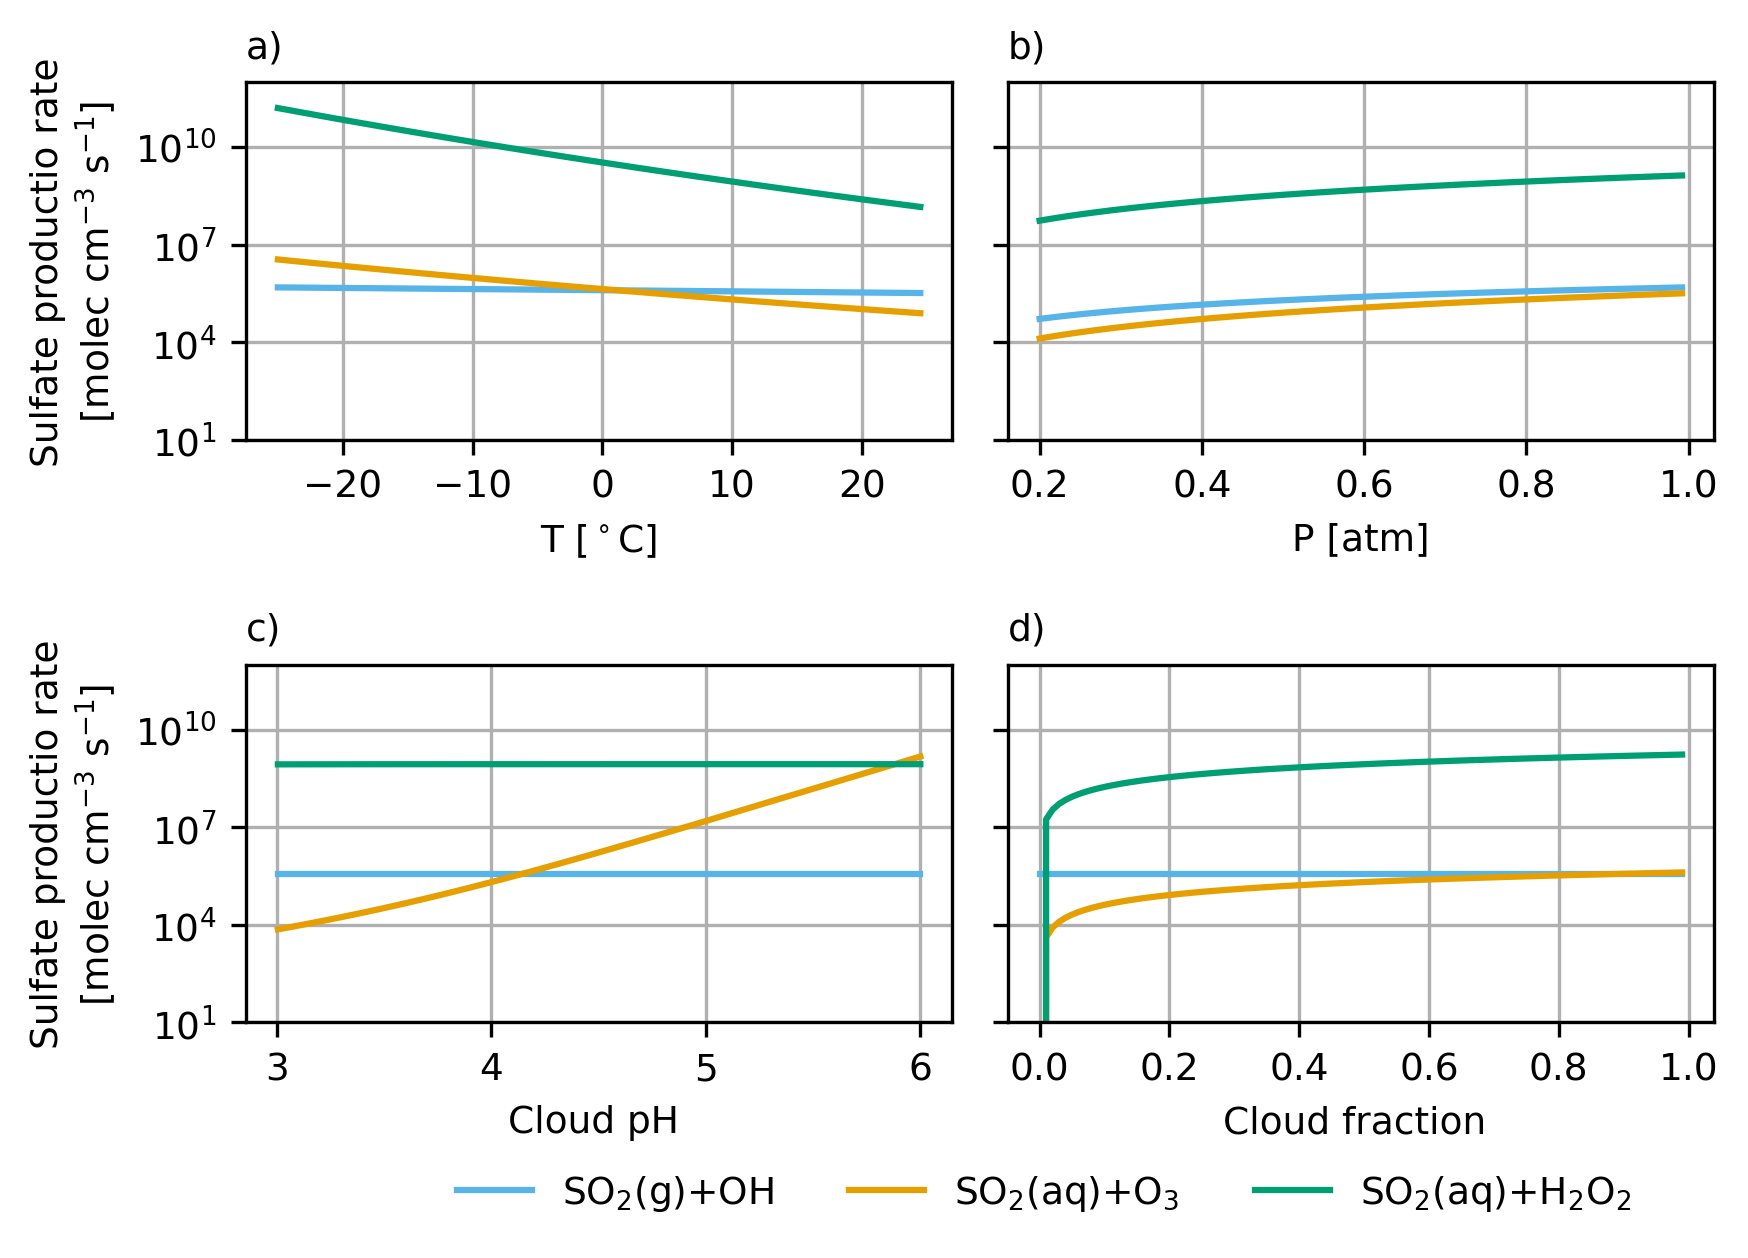
\includegraphics{Chapter4/Figs/oxidation_sensitivity.png}
    \caption[\ce{SO2} oxidation sensitivity analysis]{\ce{SO2} oxidation sensitivity analysis for a) atmospheric temperature, b) pressure, c) cloud pH and d) cloud fraction. All parameters used are shown in Table \ref{ch4:tab:sensitivity-test}}
    \label{fig:ch4:oxidation-sensitivity}
\end{figure}

\begin{figure}
    \centering
    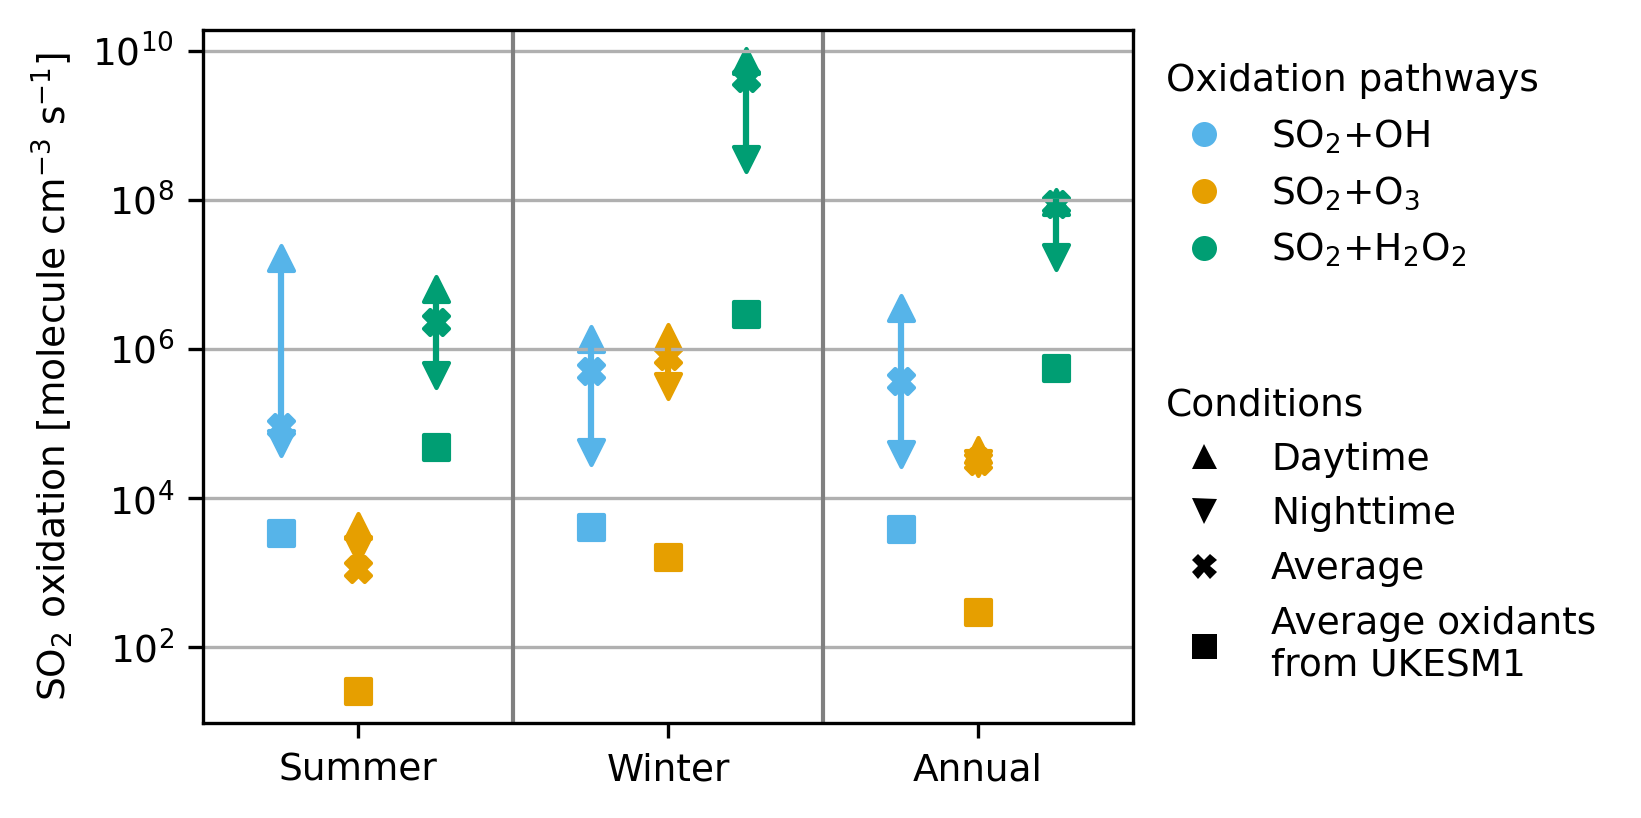
\includegraphics{Chapter4/Figs/theoretical_oxidation.png}
    \caption[\ce{SO2} oxidation calculated for summer, winter, and average conditions]{\ce{SO2} oxidation calculated for summer, winter, and average conditions as given in Table \ref{ch4:tab:sensitivity-test}}
    \label{fig:ch4:sensitivity-summary}
\end{figure}

\subsubsection{\ce{SO2} budget by season}


\begin{figure}
    \centering
    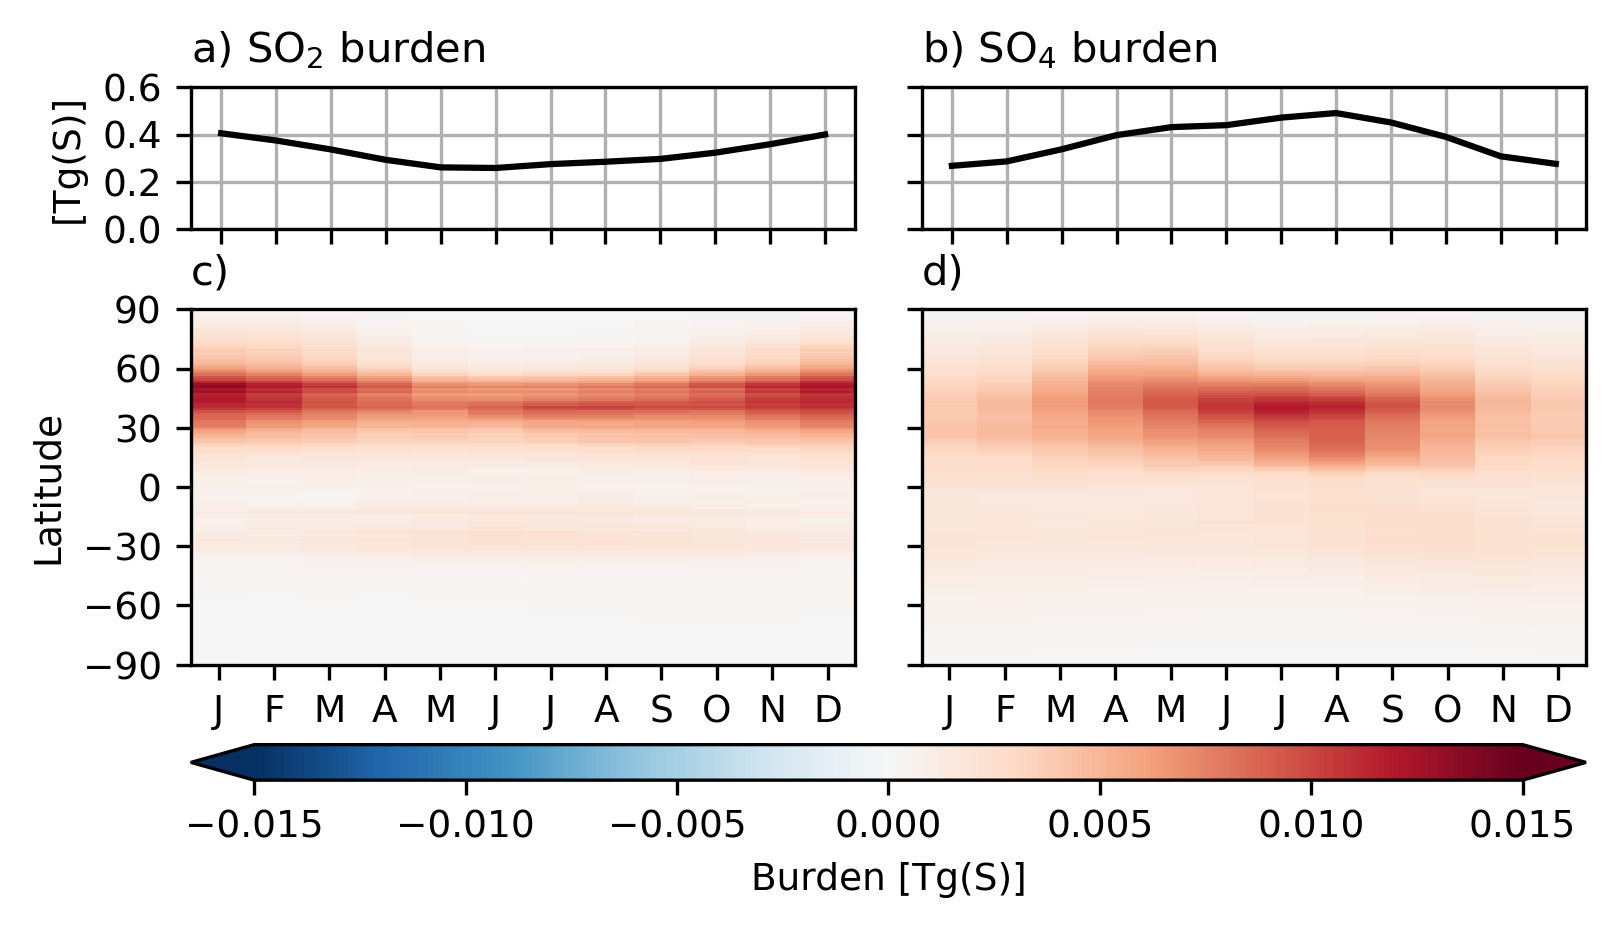
\includegraphics{Chapter4/Figs/seasonal_s_burden_1980.png}
    \caption[\ce{SO2} and \ce{SO4} mass burden by season between 1980 and 1989]{\ce{SO2} and \ce{SO4} mass burden by season between 1980 and 1989 due to aerosol precursor emissions.}
    \label{fig:ch4:seasonal-s-burden}
\end{figure}


\subsection{Seasonal cycle of aerosol properties due to aerosol precursors}


\subsection{Seasonal cycle of cloud properties}


\subsection{Seasonal cycle of aerosol ERF}
Figure \ref{fig:ch4:seasonal-erf} shows ERF between 1980-1989 averaged by month and longitude.  ERF shows a strong seasonal cycle with a high negative in the boreal summer between 1980 and 1989 where aerosol precursor emission is from Europe and Northern America. Aerosol seems to have no radiative impacts in boreal winter even though SO2 emission is the highest in winter over the same region.

\begin{figure}
    \centering
    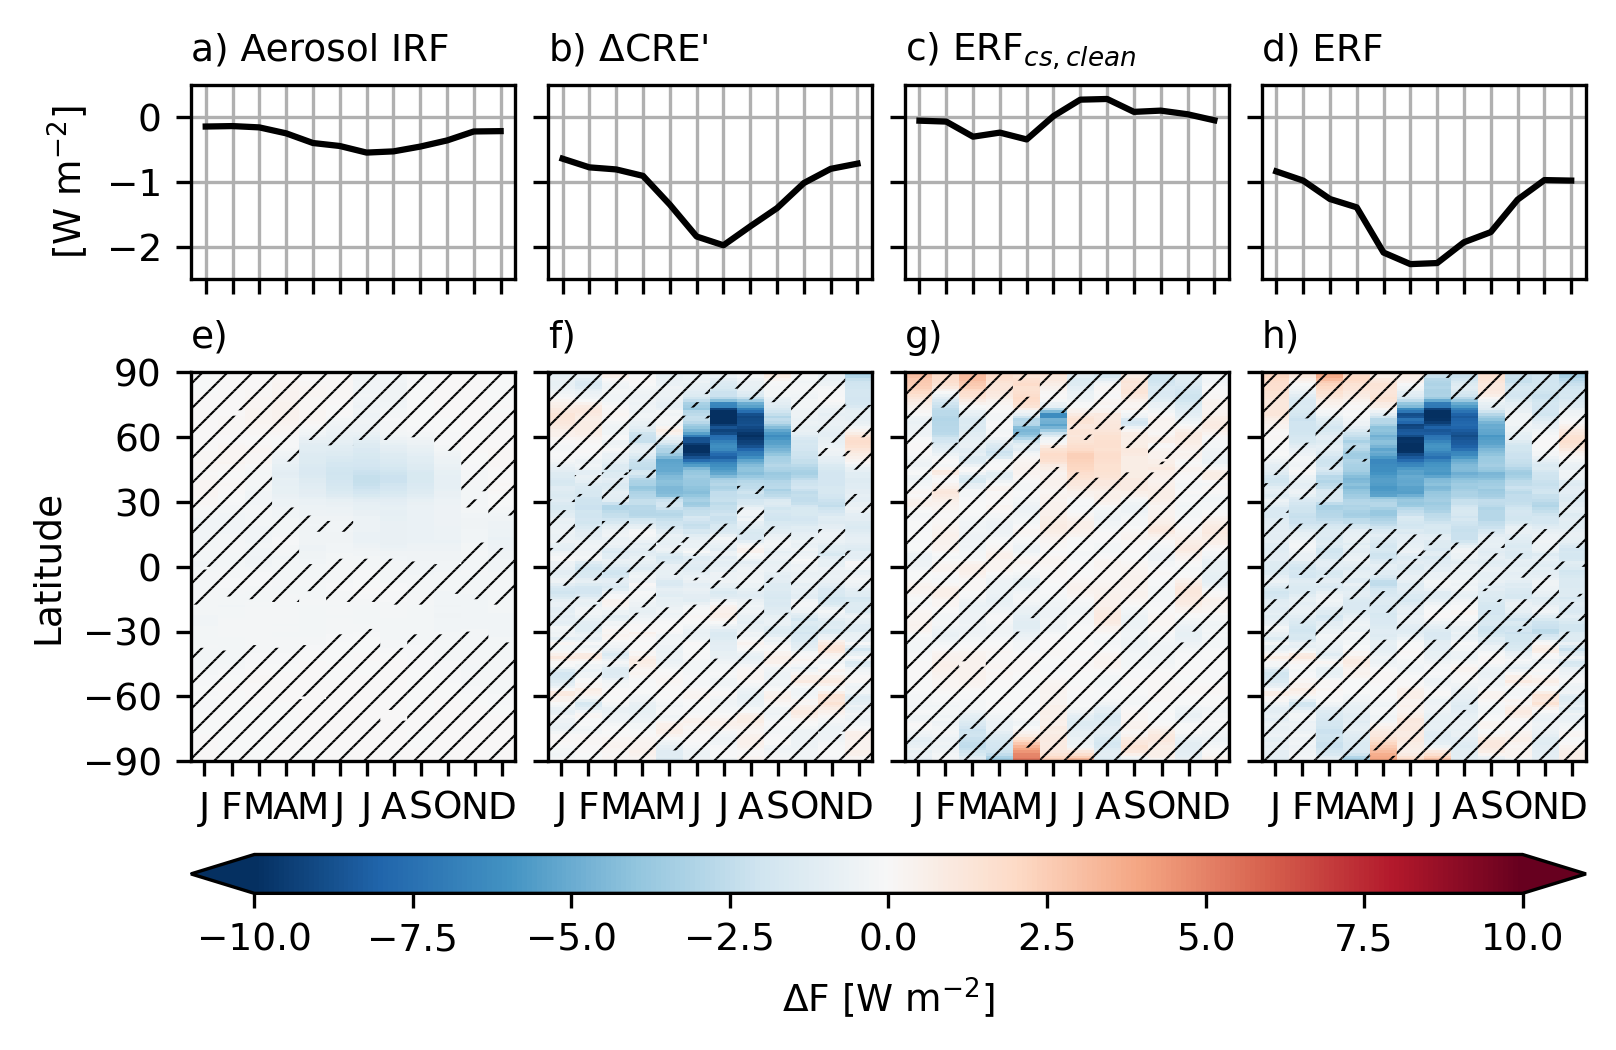
\includegraphics{Chapter4/Figs/seasonal-erf-piaer.png}
    \caption{Aerosol ERF plotted as a function of month of year and latitude between 1980-1990. Each data point is averaged longitudinally, giving 10 data points for each month and latitude. Hatch denotes points where no significant difference exists between experiment and control runs (p$\leq$0.05).}
    \label{fig:ch4:seasonal-erf}
\end{figure}


This is an important result because this implies that SO2 emitted in different seasons leads to non-linear changes in radiation.

From Chapter \ref{ch3}, we know that oxidation controls aerosol properties and subsequent radiative effects. To understand this behaviour, it is imperative to investigate the seasonal cycle of SO2 oxidation over the same period.

\section{Conclusions}